\chapter{Egyszerű számítások a munkalapon}
\thispagestyle{empty}

\section{Aritmetikai operátorok használata}

A Calc az egyenlő jellel (=) kezdődő matematikai
kifejezést kiszámítja és a cellában az eredményt
megjeleníti.

Az ,,=45*9+789'' beírásának 1194
lesz az eredménye. Aktívvá téve ismét a B2-es cellát a
\textbf{Képlet} eszköztár \textbf{Névdoboz}ában látjuk a
cella címét, a \textbf{Beviteli sor}ban pedig a kifejezést 
(\ref{AritmetikaiOperátorok} ábra).

\begin{figure}[!h]
\begin{center}
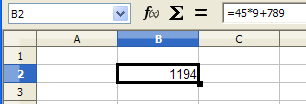
\includegraphics[width=7.094cm]{oocalcv1-img20.png}
\caption{Aritmetikai operátorok}\label{AritmetikaiOperátorok}
\end{center}
\end{figure}

A számtani alapműveletek (például összeadás, kivonás,
szorzás, osztás) végrehajtásához, számok
kombinálásához és számeredmények előállításához
az alábbi számtani műveleti jeleket használhatjuk:

\begin{description}
\item [+] (pluszjel) Összeadás;
\item [-] (mínuszjel) Kivonás; 
\item [-] (mínuszjel) Negálás; 
\item [*] (csillag) Szorzás; 
\item [/] (törtjel) Osztás;
\item [\textasciicircum] (kalap) Hatványozás (pl. 3\^{}2 --  három a négyzeten). 
\end{description}

Amennyiben egyetlen képletben több műveleti jelet vagy
operátort adunk meg, a Calc a műveleteket a következő
sorrendben hajtja végre: hatványozás, szorzás és osztás,
összeadás és kivonás. A képlet azonos prioritású
műveleteit (például szorzás és osztás) a  Calc balról
jobbra haladva értékeli ki.

A végrehajtási sorrend módosításához az elsőnek
kiértékelni kívánt képletrészt írjuk zárójelek
közé. Például az =5+2*3 eredménye 11 lesz, mivel a Calc a
szorzást az összeadás előtt hajtja végre. A képlet
összeszorozza a 2-t a 3-mal, majd hozzáad 5-öt.

Amikor a képletet módosítva zárójeleket használunk =(5+2)*3,
akkor a Calc összeadja az 5-öt és a 2-t, majd az eredményt
megszorozza 3-mal, melynek a végeredménye 21.

\section{Cellahivatkozások alkalmazása}

Legtöbbször a cellákba nem konkrét számokat, hanem
cellahivatkozásokat írunk. Módosítsuk a B2 cella tartalmát a
számok helyett az A1, B1 és C1 cellacímeket írva. Ebbe a
három cellába írjuk a kifejezés számértékeit (\ref{Cellahivatkozások}
ábra).

\begin{figure}[!h]
\begin{center}
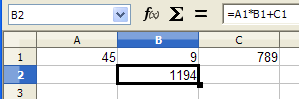
\includegraphics[width=6.909cm]{oocalcv1-img21.png}
\caption{Cellahivatkozások}\label{Cellahivatkozások}
\end{center}
\end{figure}
Módosítva az A1, B1 vagy a C1 cellák valamelyikét, a Calc
újraszámítja a cellahivatkozást tartalmazó cellát,
esetünkben a B2-t.

\section{2. feladat}
{\itshape
Készítsünk táblázatot, ami kiszámítja az A1 és a B1
cellákba írt két szám összegét, különbségét,
szorzatát és hányadosát (\ref{2-feladat} ábra)! Végezzük el az
ábrán látható formázásokat is! Ellenőrizzük az
eredményeket a következő számpárokkal: 10, 2; 81, 9 és 8,
0. Figyeljük meg a hibaüzenetet az utolsó számpár esetén a
D4 cellában. }


\begin{figure}[!h]
\begin{center}
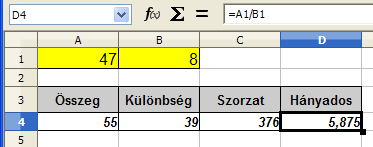
\includegraphics[width=8.867cm]{oocalcv1-img22.png}
\caption{2. feladat}\label{2-feladat}
\end{center}
\end{figure}
\section{Képletek másolása}

Táblázatos adatok esetén gyakran előfordul, hogy valamelyik
sort vagy oszlopot hasonló módon kell kiszámítani. Ilyen
esetben a képletet csak egyszer kell begépelnünk, és azt
másolással sokszorosíthatjuk.

Nevezzük át a Munkalap3 munkalapot \textbf{ZH 2}-re és
másoljuk ide az 1. feladat szegélyezett cellatartományát. Ehhez
jelöljük ki a B3:G9 tartományt, és válasszuk a
\textbf{Standard} eszköztár \textbf{Másolás} parancsát.
Ezután váltsunk a  \textbf{ZH 2} munkalap A1 cellájára és
kattintsunk a \textbf{Beillesztés} ikonra ugyanezen az
eszköztáron. Egyesítsük a G1:G3 cellákat, ebbe kerüljön
az Összesen szöveg. Végezzük el \aref{2-feladatFormázás} ábrán látható
formázásokat.

\begin{figure}[!h]
\begin{center}
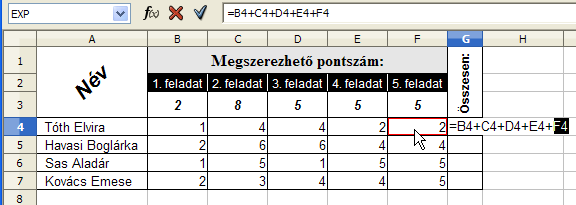
\includegraphics[width=14.238cm]{oocalcv1-img23.png}
\caption{2. feladat --  Formázás}\label{2-feladatFormázás}
\end{center}
\end{figure}

A G4 cellában számítsuk ki az első tanuló
összpontszámát. A képletben szereplő cellahivatkozásokat
egérrel is létrehozhatjuk egyszer kattintva az adott cellára. Ez
általában gyorsabb módszer, mintha a cellák címeit
gépelnénk be.

Az első tanuló összpontszámát a =B4+C4+D4+E4+F4
képlettel\footnote{Természetesen létezik a Calcban ennél
egyszerűbb megoldás is a cellatartomány összegének
kiszámítására, amit a  függvények bemutatásánál
tárgyalunk.} számítjuk ki. A második  képletet már nem
kell beírnunk, másolás segítségével létrehozhatjuk. Ehhez
vezessük az egérmutatót az aktív G4 cella jobb alsó
sarkába. Ott az keresztté változik és az egér gombját
lenyomva tartva töltsük ki (húzzuk lefelé) a G5:G7
tartományt. (\ref{2-feladatÖsszegzés} ábra)

\begin{figure}[!h]
\begin{center}
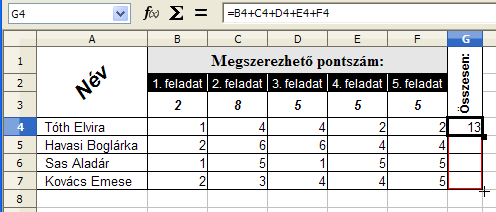
\includegraphics[width=12.122cm]{oocalcv1-img24.png}
\caption{2.  feladat --  Összegzés}\label{2-feladatÖsszegzés}
\end{center}
\end{figure}

A Calc minden cellában a megfelelő képletet hozza létre, mert
a cellahivatkozásokat tartalmazó képletet lefelé úgy
másolja, hogy növeli eggyel a cellahivatkozásokban a sorszámot.
Fölfelé másolásnál csökkenti. Az összpontszámokat úgy
is kiszámolhattuk volna, hogy először a 7. sorban lévő
képletet írjuk be, és azt másoljuk fölfelé.

Jobbra másolásnál az oszlopazonosítót ,,növeli'', ha balra másolunk,
csökkenti azt.

Amennyiben egy cella cellahivatkozásokat és számokat is tartalmaz,
akkor a képlet másolásakor az állandók nem változnak.
Például, ha egy cella tartalma =5*C1*D2+12, akkor azt lefelé
másolva   =5*C2*D3+12-t kapunk.

\clearpage
\section{3. feladat}
{\itshape
Válaszoljuk meg a következő kérdéseket, majd
ellenőrizzük a Calc segítségével:}

{\itshape
a) Az A1 cella tartalma =D3*2. Mi lesz az E5 tartalma, ha az A1 cellát
lefelé három, majd négy cellán át jobbra másoljuk?}

{\itshape
b) Az A1 cella tartalma =A8+B8-412. Mi lesz a C2 tartalma, ha az A1-et
lefelé eggyel, majd két cellán át jobbra másoljuk?}


\section{Abszolút hivatkozás}

Az eddig tárgyalt cellahivatkozásokat relatív hivatkozásoknak
nevezzük. Ez azt jelenti, hogy az ilyen hivatkozások a képletek
másolásánál automatikusan módosulnak. Vannak esetek viszont,
amikor olyan képletre van szükségünk, amelyikben egy vagy
több hivatkozás nem változik másoláskor. Ilyenkor abszolút
cellahivatkozást kell használnunk.

Abszolút hivatkozás az, ha egy az oszlop- és sorazonosító
elé egy \$ jelet írunk. Például: \$B\$3. Ez a hivatkozás
ugyanúgy a B3-as cellára mutat, de ha így szerepel a
képletekben, akkor másoláskor nem változik.

A következő feladatban áttekintjük az abszolút
cellahivatkozás használatát.

\section{4. feladat}

{\itshape
\Aref{4-feladat} ábrán egy üzletben eladott péksütemények napi adatait
látjuk. Számítsuk ki a bevételt minden napra és a heti
összbevételt is. A 8. sorban a képleteket másolással hozzuk
létre!}

\begin{figure}[!h]
\begin{center}
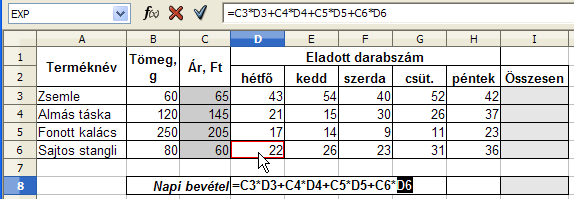
\includegraphics[width=15.185cm]{oocalcv1-img25.png}
\caption{4. feladat}\label{4-feladat}
\end{center}
\end{figure}

Szúrjunk be egy új munkalapot és nevezzük át Bevétel-re. A
hétfői bevétel kiszámítását látjuk az ábrán:
összeadjuk az egyes termékek eladásából befolyt összegeket,
amelyeket a darabszám és az ár szorzataként kapunk meg. Ezt a
képletet jobbra másolva hibás eredményt kapnánk. Ahhoz, hogy
a másolás helyes képletet hozzon létre, módosítanunk kell a
D8 tartalmát úgy, hogy az árakat megadó cellahivatkozások ne
módosuljanak. A helyes képlet tehát:
\textsf{\textbf{=\$C\$3*D3+\$C\$4*D4+\$C\$5*D5+\$C\$6*D6}}.
A \$ jeleket be is írhatjuk (AltGr+É a billentyűzeten), de
sokkal gyorsabb megoldás, ha az adott cellahivatkozásra kattintva
megnyomjuk a Shift+F4 billentyűkombinációt. A képletet jobbra
másolva így már helyes eredményt kapunk (\ref{4-feladat-2} ábra).

\begin{figure}[!h]
\begin{center}
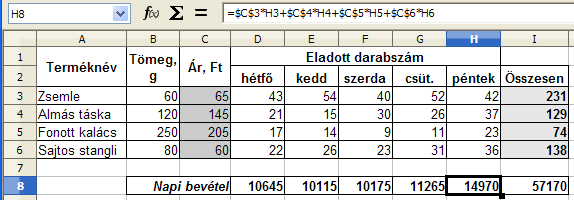
\includegraphics[width=15.185cm]{oocalcv1-img26.png}
\caption{4. feladat}\label{4-feladat-2}
\end{center}
\end{figure}


\section{Vegyes cellahivatkozások}

Relatív és abszolút cellahivatkozásokon kívül léteznek
még vegyes cellahivatkozások is. A vegyes cellahivatkozás
tartalma abszolút oszlop és relatív sor, vagy abszolút sor és
relatív oszlop. Ilyen hivatkozásokra akkor van szükség, ha azt
akarjuk, hogy a hivatkozás egyik összetevője (az oszlop- vagy
sorazonosító) állandó maradjon, a másik viszont változzon
másoláskor. Példa a vegyes hivatkozásra: =A\$1 vagy =\$A1. A
Shift+F4 billentyűkombinációt többször lenyomva
cellahivatkozás beírásakor az abszolútra, vegyesre és ismét
relatívra változik.

A vegyes hivatkozások begyakorlására készítsük el a
következő feladatot.

\section{5. feladat}
{\itshape
Hozzuk létre a természetes számok négyzeteinek táblázatát
10-től 99-ig. A képletet csak egy cellába írjuk be, a
többit másolással töltsük fel.}

\begin{figure}[!h]
\begin{center}
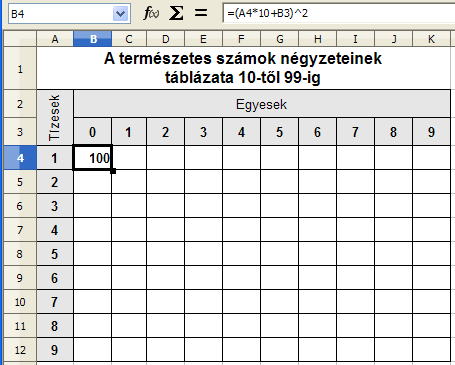
\includegraphics[width=10.037cm]{oocalcv1-img27.png}
\caption{5. feladat}\label{5-feladat}
\end{center}
\end{figure}

Új munkalapon hozzuk létre \aref{5-feladat} ábrán látható
táblázatot. Állítsuk be a cellaformátumokat. Figyeljük meg
a C4 cellába írt képletet. A képlet helyes, de jelenlegi
formájában nem másolható. Vízszintes másoláshoz úgy
kell módosítani, hogy az A4 cellacím, ami 4-es sorban tízesek
számát tartalmazza, ne változzon. Viszont ha függőlegesen
lefelé másoljuk az A4 cellacímnek A5-re kell  változnia.
Tehát az A4 cellahivatkozásban az oszlopazonosítónak
abszolútnak kell lennie, a sorazonosítónak pedig vegyesnek: \$A4.

Hasonlóképpen a B3 cellahivatkozás jobbra másoláskor
változnia kell (relatív oszlopazonosító), de lefelé
történő másoláskor nem változhat (abszolút
sorazonosító): B\$3.

Megállapíthatjuk, hogy a helyes képlet esetünkben:
\textsf{\textbf{\textcolor[rgb]{0.5019608,0.0,0.0}{=(\$A4*10+B\$3)\^{}2}}}.

Másoljuk a képletet jobbra (\ref{5-feladat-2} ábra).

\begin{figure}[!h]
\begin{center}
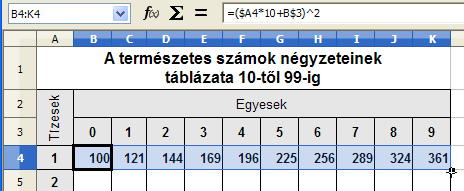
\includegraphics[width=12.275cm]{oocalcv1-img28.png}
\caption{5. feladat}\label{5-feladat-2}
\end{center}
\end{figure}

A kapott sort másoljuk lefelé, megkapva mind a 90 cellában az
eredményt (\ref{5-feladat-3} ábra).

\begin{figure}[!h]
\begin{center}
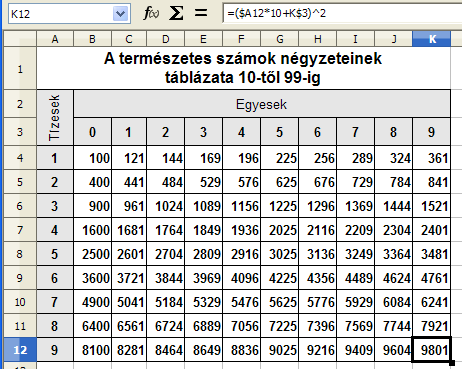
\includegraphics[width=12.222cm]{oocalcv1-img29.png}
\caption{5. feladat --  megoldás}\label{5-feladat-3}
\end{center}
\end{figure}

Térjünk vissza az előző, 4. feladatra. A D8 cellában
kiszámított hétfői bevételt jobbra másoltuk. Ilyenkor
csak a cellahivatkozás oszlopazonosító része változik.
Tehát a képletben a sorazonosítók előtti dollárjel
fölösleges. A képlet helyes eredményt ad, de --  szigorúan
véve --  itt is vegyes hivatkozást kellett volna alkalmazni. A
képlet helyesen:
\textsf{\textbf{=\$C3*D3+\$C4*D4+\$C5*D5+\$C6*D6}}.

A vegyes és az abszolút cellacímzés begyakorlására oldjuk
meg a következő feladatot.

\section{6. feladat}
{\itshape
\Aref{6-feladat} ábrán egy társasház lakásainak adatait látjuk.
Számítsuk ki a lakások havi közös költségeit, ha az a
következő összetevőkből áll:
négyzetméterenkénti alapdíj, víz és csatorna díj és
felújítási díj. A liftdíj állandó minden hónapban és
nem függ a lakás területétől. A D3 cellába írt képlet
legyen másolható minden lakásra és hónapra!}

\begin{figure}[!h]
\begin{center}
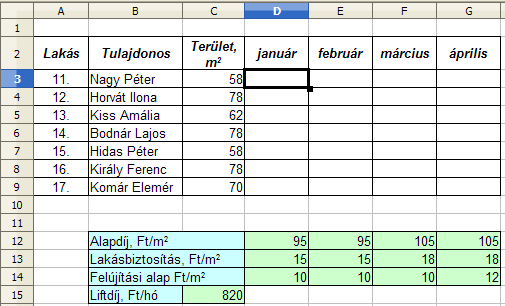
\includegraphics[width=12.813cm]{oocalcv1-img30.png}
\caption{6. feladat}\label{6-feladat}
\end{center}
\end{figure}

Az első lakás területét a C3 cella tartalmazza, a januári
költségeket pedig a D12, D13 és D14 cellák. A liftdíjat a C15
cella. A közös költséget tehát a következő képlettel
határozhatjuk meg:
\textsf{\textbf{=C3*(D12+D13+D14)+C15}}. Ahhoz, hogy
ez a képlet másolható legyen mind jobbra, mid lefelé
határozzuk meg a hivatkozások típusait. Mivel a liftdíj minden
hónapban és minden lakásra állandó,  a C15-nek abszolútnak
kell lenni. Jobbra másolásnál a születendő képleteknek
ugyanarra a lakásra  kell hivatkoznia, lefelé másolásnál
pedig a következőre. Tehát itt vegyes hivatkozást
alkalmazunk: \textsf{\textbf{\$C3}}. A díjak
esetén pedig fordítva kell eljárnunk, a vegyes hivatkozásban az
oszlopazonosítónak változni kell, a sorazonosító pedig
állandó. A végleges képlet tehát:
\textsf{\textbf{=\$C3*(D\$12+D\$13+D\$14)+\$C\$15}}. 
Figyeljük meg, hogy ez a képlet csak ilyen
hivatkozásokkal másolható a D3:G9 tartományon, bármelyik
hivatkozás módosítása hibás értékeket eredményezne.

A feladat megoldása \aref{6-feladatMegoldás} ábrán látható.

\begin{figure}[!h]
\begin{center}
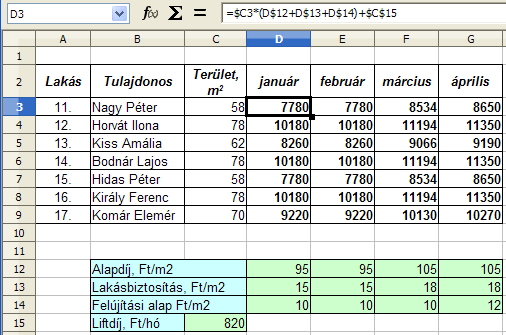
\includegraphics[width=13.386cm]{oocalcv1-img31.png}
\caption{6. feladat --  megoldás}\label{6-feladatMegoldás}
\end{center}
\end{figure}

